\chapter{Propulsion system}
\label{chap:10}
\section{Engine cycle}
\qquad The spacecraft uses electrically-driven turbo pumps to feed the oxidizer as well as the fuel to the engine. The propellant and oxidizer are each driven out of their tanks at low pressure, where after a turbo pump in each propellant line strain raises their pressures. As the oxidizer strain has a higher mass flow rate and faces a large pressure drop in the catalyzer, the respective pump is also more powerful as a result. The turbo pumps are driven electrically by electric motors which use large batteries for their power intake. These batteries offer enough charge for one maximum burn time of 900 seconds, after which they are re-powered by a fuel cell which runs on hydrogen and the hydrogen peroxide decomposition product oxygen. This will be explained further in \autoref{sec:10-3}. In order to demonstrate how exactly the engine cycle is made up, a flow schematic is shown in the following. Firstly, the pressurization system is shown in \autoref{fig1}.
\begin{figure}[H]
	\centering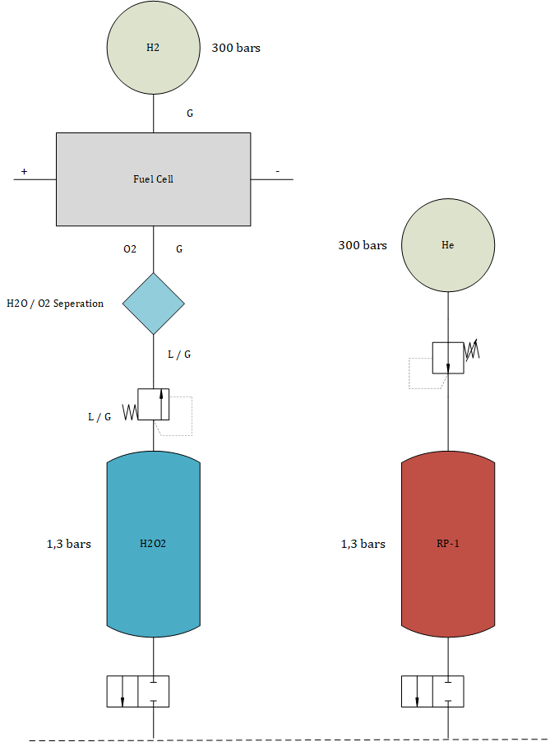
\includegraphics[width=0.5\linewidth]{pressurizationsystem}
	\caption{Flow Schematic - Pressurization system}\label{fig1}
\end{figure}

As the figure shows, only the RP-1 tank is pressurized by pressurization gas, using a $300$ bars helium tank. The hydrogen peroxide has certain decomposition characteristics which enable it to self-pressurize due to the rising pressure upon vaporization. The critical point of hydrogen peroxide is at around $150$ degrees Celsius and $1.5$ bars, meaning that if the thermal control is sufficiently reliable, a tank pressure of around $1.3$ bars can be maintained by self-pressurization. The control system and more details will be explained in \autoref{sec:10-3}. The $300$ bars H2 Tank that can be seen in the pressurization system flow schematic is therefore not a pressurization tank, but a tank for the sole purpose of running the fuel cell in combination with the oxygen which is separated from water, which is the second decomposition product of hydrogen peroxide. The separation works by simply condensing the water and allowing the gaseous oxygen to pass through a filter. Both the RP-1 tank and the H2O2 tank have a main valve after their outlets, which are visible in \autoref{fig1}. The remaining feeding system is shown in the second part of the flow schematic, depicted in \autoref{fig2}.

\begin{figure}[H]
	\centering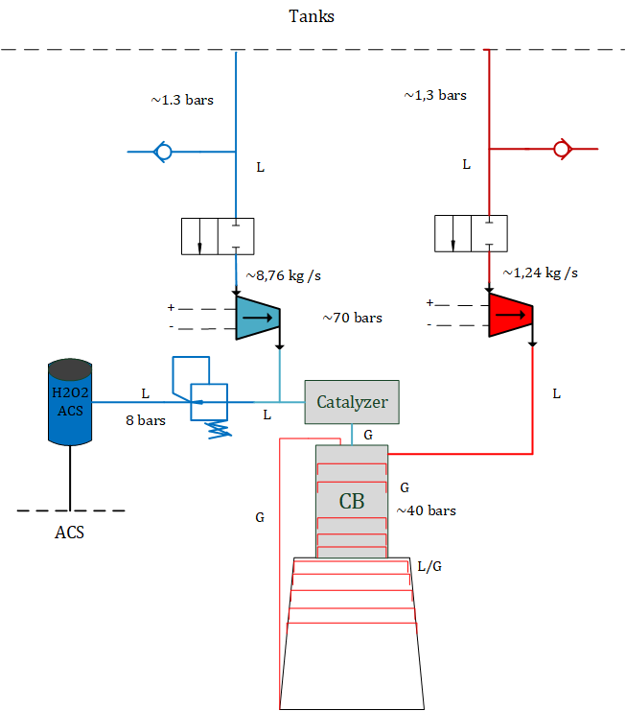
\includegraphics[width=0.7\linewidth]{flowenginesection}
	\caption{Flow Schematic - Engine section}\label{fig2}
\end{figure}
The fueling ports for RP-1 as well as hydrogen peroxide extend to the left- and right-hand-side of the top of the figure. Check valves are situated at these points to only allow propellant flowing in. A second main valve for both propellants is installed just before the turbopumps, which are closed during refueling. While the RP-1 is then funneled through cooling channels in the regenerative cooling system, the oxidizer runs into a catalyzer, where a rapid decomposition reaction splits the hydrogen peroxide into its reactive products for combustion. A second oxidizer strain is guided towards a pressure regulation valve, behind which it continues into a buffer tank of hydrogen peroxide for monopropellant use in the ACS. The catalyzers for ACS thrusters are located in close proximity to their respective combustion chambers. The ACS is not depicted as a flow schematic.

\section{RCS / ACS}

In the previous section we mention that we are going to use hydrogen peroxide as a monopropellant for our Reaction Control System. Indeed, hydrogen peroxide can be used as a quite good RCS propellant. \\

At the moment, the biggest part of the monopropellant thruster using $H_2O_2$ are test bench engine. This is because of the difficulty to characterize the engine and its parameters. \\

Hydrogen peroxide is usable as a monopropellant because of its natural decomposition. As we are going to see on the Catalyzer part further on the report $H_2O_2$ can be decomposed in $H_2$ and $H_2O$. That's this decomposition we are going to use inside our thruster. \\
When hydrogen peroxide goes through a catalyser it decomposes and generates a great amount of heat, up to $1000K$. This two factors create steam at a very high temperature and pressure; it's this steam that creates our thrust.\\

Before designing the engine and its characteristics we need to choose the positioning of the thrusters. In order to do that, we based our design on the American Space Shuttle which use cluster of small thrusters all around the spacecraft to allow a good maneuverability.  

\begin{figure}[H]
    \centering
    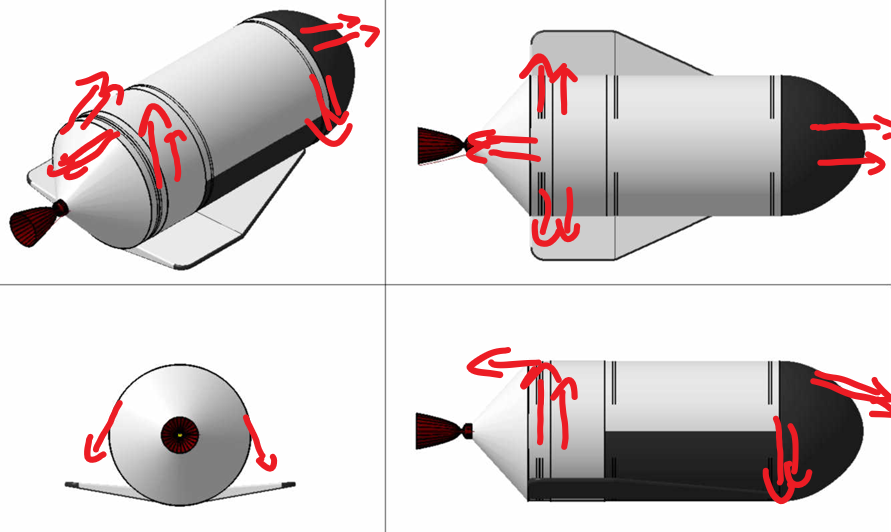
\includegraphics[width=\linewidth]{shiprcs}
    \caption{RCS thruster repartition}
\end{figure}

We are going to use 6 different clusters spread over the craft, each cluster is composed of 2 thrusters for a total of 12. This disposition allow to manipulate every axis. \\

Now we need to compute the characteristic of the thruster, to do so we used RPA (a NASA software to compute the parameters of a thruster based on the propellant and several other characteristics) and some papers of recent studies about hydrogen peroxide thruster. \\

We assumed a chamber pressure of $10bars$ and a thrust of $100N$, then we use RPA to get the other parameters.

\begin{itemize}
    \item Combustion temperature: $1223K$
    \vspace{-0.4cm}
    \item Ejection temperature: $424K$
    \vspace{-0.4cm}
    \item Ejection pressure : $0.094bars$
    \vspace{-0.4cm}
    \item $\gamma = 1.335$
    \vspace{-0.4cm}
    \item $R = 368.6$
    \vspace{-0.4cm}
    \item $ISP = 140s$
\end{itemize}

With these parameters we can then compute every other parameters we want for the thruster and especially the mass flow rate which is necessary to have a correct mass budget. 

$$c^* = \sqrt{\frac{R T_c}{\gamma}}\times \frac{\gamma + 1}{2}^{\frac{\gamma + 1}{2(\gamma - 1)}}$$

Throat characteristics:
$$T_t = T_c \left(\frac{2}{\gamma + 1}\right) \hspace{20pt}
P_t = P_c \left(\frac{2}{\gamma + 1}\right)^{\frac{\gamma}{\gamma - 1}} \hspace{20pt}
\rho = \frac{P_t}{R T_t} \hspace{20pt}   u_t = \sqrt{\gamma R T_t}$$

Exhaust characteristics:
$$M_e = \sqrt{\frac{2}{\gamma - 1}\left[\left(\frac{P_c}{P_e}\right)^\frac{\gamma - 1 }{\gamma} - 1 \right]} \hspace{20pt} T_e = \frac{T_c}{1 + \frac{\gamma - 1}{2}M_e^2}  \hspace{20pt} \rho_e = \frac{P_e}{R T_e}$$

\clearpage

Thus we can compute the area ratio and the thrust coefficient:

$$\frac{A_e}{A_t}= \frac{1}{M_e}\left[\frac{2}{\gamma + 1}\left(1 + \frac{\gamma - 1}{2} M_e^2 \right)\right]^{\frac{\gamma + 1}{2(\gamma - 1)}}$$

$$ C_F = \gamma \sqrt{\left(\frac{2}{\gamma + 1}\right)^{\frac{\gamma + 1}{\gamma - 1}}\frac{2}{\gamma - 1} \left[ 1 - \left(\frac{P_e}{P_c}\right)^{\frac{\gamma - 1}{\gamma}}\right]} + \frac{P_e - P_a}{P_c}\frac{A_e}{A_t} $$ 

\vspace{0.5cm}

Finally we can compute the exhaust velocity, throat area and the mass flow: 

$$c = C_F c^* \hspace{20pt} A_t = \frac{F}{C_F P_c} \hspace{20pt} \dot m = \frac{P_c A_t}{c^*}$$

Thus we can write the following Matlab code to simulate:

\begin{minted}[linenos, autogobble, breaklines]{matlab}
Pc = 10; % Chamber pressure
Pe = 0.094; % exhaust Presssure (given RPA)
gamma = 1.335; % RPA
R = 0.3686e3; % RPA
Tc = 1223; % Combustion temperature given (RPA)

c = sqrt( R * Tc / gamma) * ((gamma + 1)/2)^((gamma + 1)/2 * (gamma - 1));

% Throat characterisctics
Tt = Tc * (2/(gamma + 1));
Pt = Pc * (2/(gamma + 1))^(gamma/(gamma -1));
rho = Pt / R * Tt;
Ut = sqrt(gamma * R * Tt);

% Exhaust characteristics
Me = sqrt((2/(gamma - 1))*((Pc/Pe)^((gamma - 1)/ gamma) -1));
Tebis = Tc / (1 + ((gamma - 1) / 2) * Me^2);
rho_e = Pe / R * Tebis;

Exp_ratio = (1 / Me) * ((2 / (gamma + 1)) * (1 + ((gamma - 1) / 2) * Me^2))^((gamma + 1)/2*(gamma-1));
Cf = gamma * sqrt((2/(gamma + 1))^((gamma + 1)/(gamma - 1)) * (2/(gamma - 1)) * (1 - (Pe/Pc)^((gamma - 1)/gamma))) + ((Pe - 1)/Pc) * Exp_ratio;

c_e = Cf * c; At = 100 / (Cf * Pc); m_flow = (Pc * At)/c;
\end{minted}

From the simulation we finally have:

\begin{itemize}
    \item Exhaust velocity: $c=617.38m/s$
    \vspace{-0.4cm}
    \item Mass flow rate: $\dot m = 0.105 kg/s$
\end{itemize}

The most important value for us is the mass flow rate as it allows us to compute the propellant mas needed to perform our maneuvers. \\


In addition of the thrusters we also need another system which is the Reaction Wheels. This systems which is separated in 3 different wheel, one for each axis, and allow to rotate the entire craft on the 3 axis with the the reaction motion applied by the rotation of the wheel.

\section{Multi-usage of hydrogen peroxide}
\label{sec:10-3}
Hydrogen Peroxide as the main engines oxidizer is the main dictator of all sub-system and system design decisions. GREDER uses it for following applications:
\begin{enumerate}
	\item	Main engine oxidizer
	\item	ACS mono-propellant
	\item	Fuel cell power generation in combination with stored hydrogen
	\item	Oxidizer tank pressurization
\end{enumerate}

Hydrogen peroxide’s decomposition behavior is the reason for its multi-purpose usability, but also its major risk. If the pressure or temperature in the tank go unregulated and exceed certain boundaries, the propellant can enter critical status and endanger the tank’s integrity. Therefore, extensive design and simulation was conducted to determine a tank design which allows thermal regulation based on the rotational angle of space craft, as indicated in \autoref{fig:tempreg}. 

\begin{figure}[H]
	\centering
	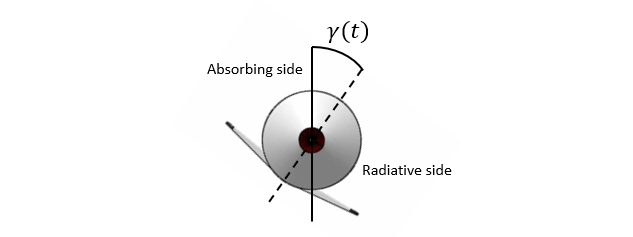
\includegraphics[width=\linewidth]{tempreg}
	\caption{Lessons learnt}\label{fig:tempreg}
\end{figure}

The absorbing side of the space craft is painted in a way which causes a high absorption coefficient and a low emissivity, while the radiative side is coated vice-versa. The tank materials are chosen to deliver high heat transfer while being compatible with hydrogen peroxide. Thereby, a rotation of the space craft will cause a change in the heat flux, while every hydrogen peroxide temperature can be assigned a rotational angle for neutral heat flux at which no temperature change happens. This design was simulated with some simplifications and its technological feasibility could be verified. This is detailed in \autoref{sec:11-3}. \\

The usage of hydrogen peroxide is the sole reason for GREDER using electrically-driven turbo pumps, as the ease in electricity production makes this the most efficient method. The relatively low combustion chamber pressure and thrust are not a major issue, as a long mission duration is necessary anyways for electricity production in between burns. In addition, the low complexity of the electric turbo pump cycle compensates for the higher complexity of the challenge of storing hydrogen peroxide for long durations, as it is a highly reactive chemical which poses extreme risks, especially due to its decomposition behavior, which GREDER uses as an advantage. \\

As batteries have a low energy density compared to chemical fuels, electric cycles for main engines usually come with a mass disadvantage due to the necessity of carrying large battery masses. While GREDER needs a total main engine burn time of around 2500 seconds per mission, the battery only needs to power the turbo pumps and electrical equipment for 900 seconds at a time, because the hydrogen peroxide decomposition product oxygen powers a fuel cell in combination with hydrogen between main engine burns for additional power generation. The main trade-off to consider at this point is between bringing a fuel cell, a hydrogen tank and the additional equipment for separation of the decomposition products and dimensioning the battery large enough for powering the entire mission. As the other applications of the hydrogen peroxide are discussed in other chapters, this chapter will detail the power generation usage and detail a trade-off with respect to using a larger battery. The detailed description of how the power generation and tank pressure control work can be found in chapter 12 and the simulation model in the annex. This chapter will use analytical terms to compare the two approaches, while the simulation can be seen as a proof of concept.\\

In order to determine the necessary masses for the additional components for fuel cell usage, the energy output of the fuel cell was calculated using the reaction energy multiplied with an assumed efficiency coefficient supported by literature. Following assumption for the efficiency was made:

\begin{equation}
	\eta_{Fuel_{cell}} = 0.6
\end{equation}
With the theoretical reaction energy being :
\begin{equation}
	P_{Fuel\ cell_{th}} = 286\ 000 \ J/mole
\end{equation}
For the reaction :
\begin{center}
	$2H_2\ +\ O_2\ =\ 2H_2O$
\end{center}

Taking the mole masses into account and assuming complete reaction, for every kilogram of hydrogen the fuel cell uses $7.937$ kg of oxygen. The resulting energy per kilogram of hydrogen can then be calculated as follows:
\begin{equation}
	E_{Fuel\ cell_{real}} = 286\ 000\ J/mole \times 0.6\times\frac{1kg}{0.01\ kg/mole} = 47.29\ kWh
\end{equation}
In order to perform a trade-off calculation between using a fuel cell for battery re-charging or installing a larger battery directly, the total masses for both systems will be compared at this point. The current mass budget for the fuel cell system is as follows:
\begin{table}[H]
	\centering
	\begin{tabular}{|c|c|}
		\hline
		Component & Mass (kg)\\
		\hline
		Battery & $388.66$\\
		\hline
		Fuel cell & $202$\\
		\hline
		$H_2$ tank & $5$\\
		\hline
		Other equipement & $10$\\
		\hline
		\cellcolor{gray!50}Total & \cellcolor{gray!50}$605.66$
	\end{tabular}
\end{table}

Now, as the fuel cell allows GREDER to only be designed for a $900$ s duration of not being re-powered, the battery mass can remain relatively low at a conservative battery energy density of $100$  Wh/kg. During the burn duration, around $98.6$\% of electrical energy is used to power the turbo pumps. Therefore, as a first estimate, the necessary battery mass for powering the turbo pumps during all mission burn times, which amount to $2475.2$ seconds, is calculated:
\begin{equation}
	m_{Bat,\ only bat} = \frac{P_{TP}\times 2475.2s}{100\ Wh/kg} = 1\ 053.9\ kg
\end{equation}

This results in a \textbf{mass difference of 448.2kg in favour of the fuel-cell architecture}. Now, two possible problems can be brought up with this estimation:
\begin{enumerate}
	\item	The energy density estimate is at the lower end of current lithium battery technology and a higher density would result in a shift towards the advantages of using only a battery.
	\item	The fuel-cell architecture is not technologically proven in combination with hydrogen peroxide decomposition and constitutes larger technical complexity.
\end{enumerate}

While these points are valid arguments for using only a battery, the trade-off analysis clearly pointed out using a fuel-cell would result in a mass reduction, the higher level of technical complexity of which is justifiable. The above-mentioned arguments can be answered as follows:
\begin{enumerate}
	\item	While lithium batteries of higher energy densities have been flight-proven, the mission itself has never been performed in a similar way. Refuelling and frequent satellite capturing are completely new territory and therefore, conservative estimates in key design criteria offer a way of compensating for the additional mission challenges.
	\item	Fuel cells are very well researched and very common technology in on-earth use. Therefore, the implementation of a decomposition-product recycling system, while posing some new design problems, is not comparable to the difficulty of challenges like designing a new engine. Additionally, as this mass estimate only takes turbo pump power into account, the battery-only architecture would need to either have even greater battery mass or be fitted with solar power generators to cover the system power requirements between burns. This again adds up to system complexity and poses large problems during re-entry.
	
\end{enumerate}
\section{Propellant tanks}
The vehicle must use propellant tanks in order to carry the oxidizer and fuel, in this case H2O2 and RP-1, during the mission. The required total useable propellant was already found in the final mass budget calculation. 
This chapter describes the tank design beginning with the requirements and tank specification, afterwards the analysis of compatible materials following by the design including different options, expulsion principle, stresses, MAIT and final design. The Liner tanks are also addressed in the last part of this chapter.\\

\subsection{Requirements and specification}
Several parameters have to be set in prior to the propellant tank design in order to ensure that all top level vehicle and propulsion system requirements are met. Additionally it must be ensured that the propellant tank assemblies sustain launch and flight loads during all phases of the mission.
\subsubsection{Propellant Tank masses and volumes}

\autoref{tab:propmass} shows the calculated values of the final propellant mass and final volumes of both oxidizer and fuel. The basis of this calculation is the final mass budget that provided the useable propellant masses. Starting at this value and calculating 1\% additional propellant for ignition, 2\% for shutdown, 2\% performance reserve and 2\% residuals, the masses add up to 24t for H2O2 and 3.4t for RP-1. H2O2 needs a greater ullage volume than RP-1 due to the decomposition, with 20\% ullage a total tank volume of $\geq$ 18.62 m$^3$ is necessary. For RP-1 a total tank volume of  $\geq3.99$ m$^3$ needs to be accomplished.
\begin{table}[H]
    \centering
    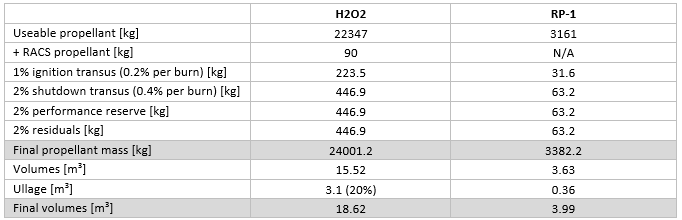
\includegraphics[width = \linewidth]{propmassvol}
    \caption{Propellant masses and volumes}
    \label{tab:propmass}
\end{table}{}
\subsubsection{Driving requirements}
The driving requirements for the oxidizer propellant tank assembly (PTA) are summarized in \autoref{tab:PTAreq}. MDP is taken according to ECSS\footnote{ECSS‐E‐ST‐32‐01C Rev. 1, Fracture control}
\begin{table}[H]
    \centering
    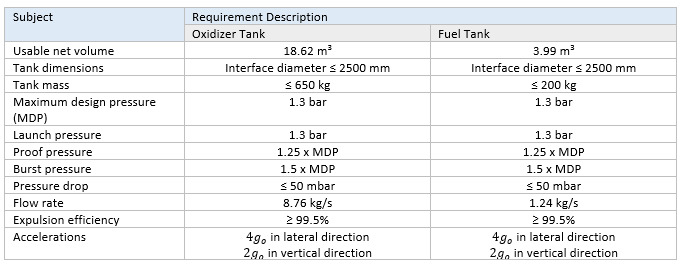
\includegraphics[width = \linewidth]{ptareq}
    \caption{PTA driving requirements}
    \label{tab:PTAreq}
\end{table}{}\pagebreak
\subsubsection{Pressure loads}
The ECSS\footnote{ECSS‐E‐ST‐32‐01C Rev. 1, Fracture control} requires a safety factor of 1.25 on proof pressure and 1.5 on burst pressure. Therefore the pressure levels including safety factors are listed in \autoref{tab:ptapress}.
\begin{table}[H]
	\centering
	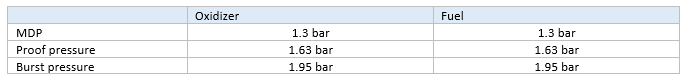
\includegraphics[width = \linewidth]{ptapress}
	\caption{PTA pressure loads}
	\label{tab:ptapress}
\end{table}{}
The number of pressure cycles after delivery is shown in \autoref{tab:ptacycle}. This number of pressure cycles applies for both the oxidizer and fuel tank.
\begin{table}[H]
	\centering
	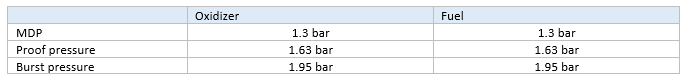
\includegraphics[width = 0.6\linewidth]{ptapress}
	\caption{PTA pressure cycles}
	\label{tab:ptacycle}
\end{table}{}
\pagebreak
\subsection{Materials}
The intended materials for the propellant tanks are listed in \autoref{tab:tankmat}. For the fuel tank and liner tanks a common titanium alloy can be used with high strength and good ductility. The titanium alloy shall be heat treated to .7 status (solution treated and aged) in order to achieve the below mentioned material characteristics and to stress relieve. The liner tanks can also be winded or wrapped with CFK in order to be further strengthened and to reduce the wall thickness of the titanium.\\

The oxidizer tank shall be manufactured of aluminum 5254 which is long term compatible and corrosion resistant against H2O2. Unfortunately the aluminum alloy shows a low strength which has to be taken into account in the mechanical calculations. A higher strength option of this alloy is currently in development acc. to NASA paper.
\begin{table}[H]
	\centering
	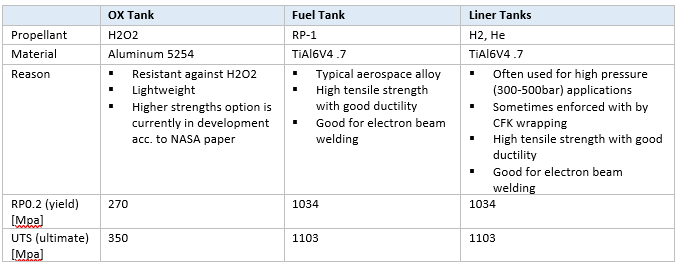
\includegraphics[width = \linewidth]{tankmat}
	\caption{Propellant tank materials}
	\label{tab:tankmat}
\end{table}{}
\pagebreak
\subsection{Concepts and options}
During the process of finding the optimum propellant tank concept for the GREDER vehicle, our mission and application, several possible design option have been taken into account. \autoref{fig:tankdesign} shows the three most promising options.\\

The first option is an integrated concept with the fuel tank placed within the oxidizer tank. Integrated designs are in theory the most lightweight design option for propellant tanks because the basic idea is to reduce the wall thickness of the inner tank due to theoretically no pressure delta between fuel and oxidizer tank pressure. The downside of this option is the manufacturing. Also the use of spacecraft volume is quite attractive with this design. Manufacturing of one tank inside of another tank and then welding it is a tough task. Additionally the fuel tank also needs to be compatible with both propellants because it is in contact with the oxidizer from the outside and the fuel from the inside. Therefore option 1 is not suitable for our application due to manufacturing complexity, material compatibility and our MDP of 1.3 bar is way too low to justify the advantage of wall thickness reduction.\\

The second option is also an integrated option but this time with two separate tanks. This slightly increases the spacecraft volume but is still more spacecraft volume efficient than option 3. This option, especially the special shape of the oxidizer tank, is a complex geometry and therefore also complex to manufacture. The fuel tank manufacturing is simpler than in the first option due to the half sphere hemispheres and gimbal mounting. During first attempts of a detailed design of that option it was found that the vehicle diameter increased over the boundary requirement. For this reason and also due to the complex manufacturing and design this option was found to not be the most efficient design for our application.\\

The third option is a rather simple “two-tanks-on-top-of-each-other” design. The main advantage is here the simple design and manufacturing and assembly of all parts, the possibility of load carrying structure of the outer tank walls as well as good options for tank expulsion principles. This design was found to be the optimum for our application and is therefore the baseline for all further calculations and detailed design.

\begin{figure}[H]
	\centering
	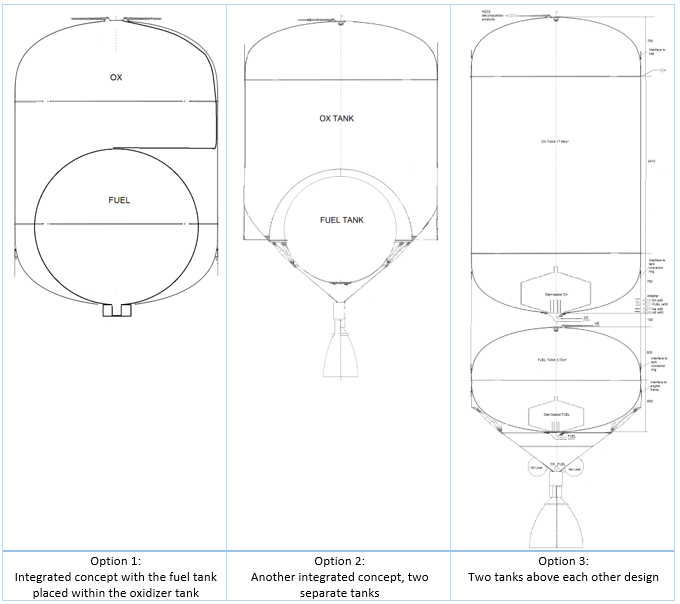
\includegraphics[width=\linewidth]{tankdesignoption}
	\caption{Different propellant tank design options}\label{fig:tankdesign}
\end{figure}
\subsection{Final design}
The final design is therefore an option with a stacked structure, as already mentioned in the previous chapter. \autoref{fig:detail} shows a detailed view on the final design with the major parts shown. The Oxidizer tank consists of two cassini shaped hemispheres and one large cylinder (or several smaller cylinders if easier to manufacture). The fuel tank is built with the same cassini hemispheres, but without a cylinder. This usage of the same hemispheres for both oxidizer and fuel tanks reduces costs for jigs and tools and also for development. Each tank has an inlet at the top of the tank and an outlet at the bottom. It has to be mentioned that the upper port of the oxidizer tank is used to extract the H2O2 decomposition products and not to pressurize the tank since the tank is self-pressurizing.

Both propellant tanks make use of start baskets, the function is explained in the subsequent chapter.\\

The propellant tanks are the carrying structure of the spacecraft and they are connected by interface connector rings. In the interface connector ring there are also the adapters for refueling planned.\\

At the bottom of the spacecraft near the engine are the liners located. There is one helium liner tank for Fuel tank pressurization and one hydrogen liner tank for the fuel cell operation.
\autoref{fig:designfull} shows a full view on the final design of the propellant tanks.
\begin{figure}[H]
	\centering
	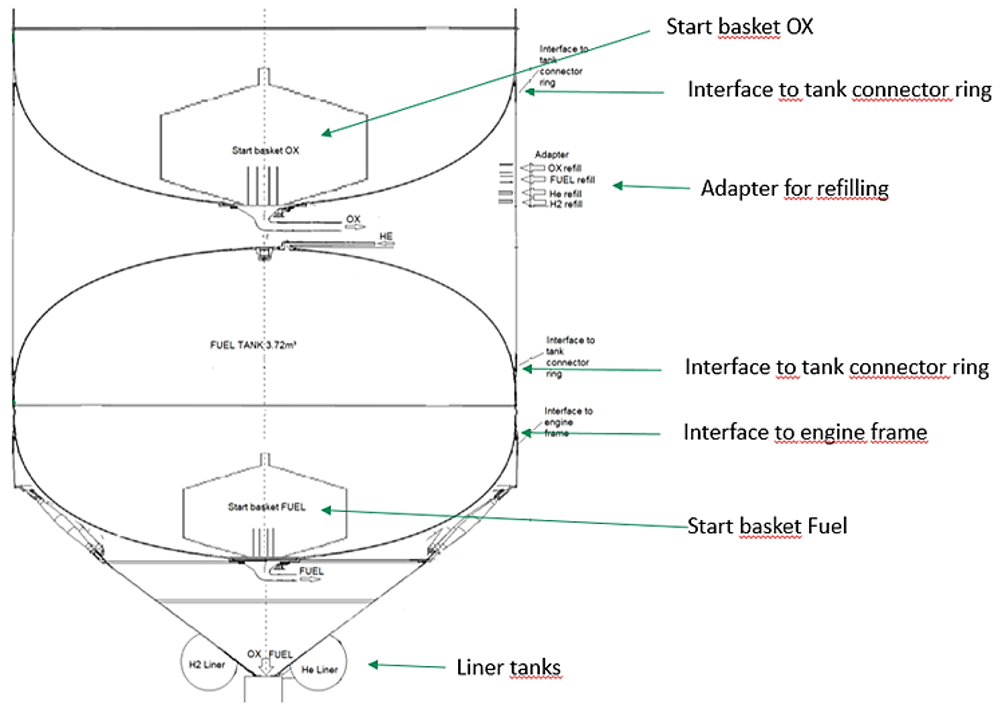
\includegraphics[width=\linewidth]{tankdetail}
	\caption{Final propellant tank design detailed view}\label{fig:detauk}
\end{figure}
\begin{figure}[H]
	\centering
	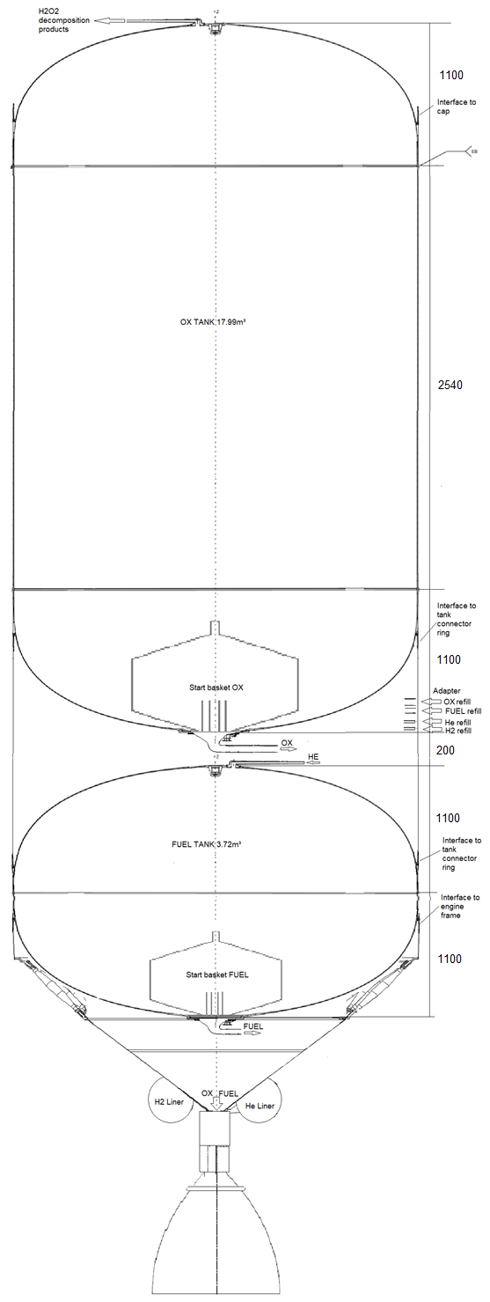
\includegraphics[width=0.4\linewidth]{tankfull}
	\caption{Final propellant tank design full view}\label{fig:designfull}
\end{figure}
\subsection{Expulsion principle}
The refillable start basket is a structure within the propellant tanks located at the outlet of the tank that is designed to ensure that there is always propellant at the outlet in zero gravity condition – at least until the spacecraft acceleration again forces the propellant towards the outlet. If the thrusting duration is sufficient to settle the liquid each time, the start basket, is the best light weight and simple propellant management device. The start basked volume for each of the tanks must be big enough (with margin) to supply propellant to the engine until acceleration settles the liquid again. Another important aspect is that the start basket must be refillable to allow several ignitions of the engine. This principle is shown in \autoref{fig:startbasket}.
\begin{figure}[H]
	\centering
	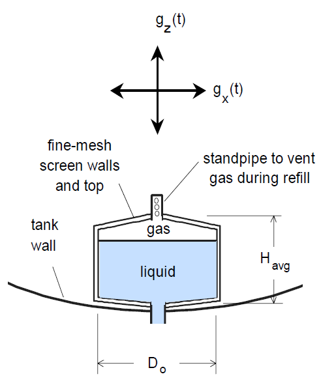
\includegraphics[width=0.3\linewidth]{startbasket}
	\caption{Final propellant tank design full view}\label{fig:startbasket}
\end{figure}
\subsubsection{Start basket design}
For the start basket design, the maximum acceleration has to be defined. As already listed in the propellant tank requirements, the maximum acceleration is:
\begin{align}
    g_x &= 4\times g_0\\
    g_z &= 2\times g_0\\
    g_0 &= 9.81 m/s
\end{align}{}

The first step for the start basket design is the calculation of settling acceleration, the acceleration with which the propellant moves towards the outlet
\begin{equation}
    a_{set} = \frac{F}{m_{spacecraft}} = \frac{32860N}{28302kg} = 1.16m/s^2
\end{equation}{}
With this acceleration the time the propellant needs to reach the ground can be calculated
\begin{align}
    t_{fall_{Oxidizer}} &= \sqrt{\frac{h_{Ox}}{\frac{1.16}{2}}} = \sqrt{\frac{4.74}{\frac{a_{set}}{2}}} =2.54s\\
    t_{fall_{Fuel}} &= \sqrt{\frac{1.2}{\frac{1.16}{2}}} = 2.54s
\end{align}{}

Since the time that the oxidizer and fuel need to reach the outlet is now known, the settling time can be calculated. The settling time is the falling time multiplied by four. This is a heritage value
\begin{align}
    t_{set_{Oxidizer}} &= 4\times t_{fall_{Oxidizer}} = 10.16s\\
    t_{set_{Fuel}} &= 4\times t_{fall_{Fuel}} = 5.76s
\end{align}
With this information, the necessary start basket volume can be calculated by calculating what propellant volumes are needed to cover the settling time while still providing the requested flow rates to the engine.
\begin{align}
    V_{basket_{Oxidizer}} &= \frac{t_{set_{Oxidizer}} \times \dot{m_{Oxidizer}}}{\rho_{Oxidizer}} = 0.0618m^3\\
    V_{basket_{Fuel}} &= \frac{t_{set_{Fuel}} \times \dot{m_{Fuel}}}{\rho_{Fuel}} = 0.0079m^3
\end{align}{}
It is now possible to roughly calculate size of the start basket by assuming it to be a cylinder with $d=h$
\begin{align}
    d_{Oxidizer} &= h_{Oxidizer} = \bigg(\frac{V_{basket_{Oxidizer}}}{\frac{4}{\pi}}\bigg)^{\frac{1}{3}} = 0.36m\\
    d_{Fuel} &= h_{Fuel} = \bigg(\frac{V_{basket_{Fuel}}}{\frac{4}{\pi}}\bigg)^{\frac{1}{3}} = 0.18m
\end{align}{}

Afterwards the screens and screen drillings have to be dimensioned in such a way that the screens are capable to hold the propellant inside of the start basked by propellant surface tension. The if the pressure on the grids due to hydrostatic pressure by $g_x$ (the highest acceleration) exceeds the bubble point pressure, the liquid will break through and is not captured inside the start basket anymore

\begin{align}
    p_{BubblePoint_{Oxidizer}} = \rho_{Oxidizer}\times g_x \times h_{Oxidizer} = 206mbar\\
    p_{BubblePoint_{Fuel}} = \rho_{Fuel}\times g_x \times h_{Fuel} = 65mbar\\
\end{align}{}
In the last step the screen drillings are dimensioned in that way that the bubble point is not exceeded by the acceleration taking the surface tension into account
\begin{align}
    Stens_{Oxidizer} &= 0.08 N/m\\
    Stens_{Fuel} &= 0.028 N/m\\
    d_{drillings_{Oxidizer}} &= \frac{4\times Stens_{Oxidizer}}{p_{BubblePoint_{Oxidizer}}} = 0.0155mm\\
    d_{drillings_{Fuel}} &= \frac{4\times Stens_{Fuel}}{p_{BubblePoint_{Fuel}}} = 0.0172mm\\
\end{align}{}
Therefore it has to be a very fine mesh. 
\subsection{Stresses}
For the preliminary calculation of stresses and wall thicknesses several loads on the propellant tank have been identified:
\begin{itemize}
    \item   Internal tank pressure
    \item	Hydrostatic pressure on tank walls due to accelerated propellant
    \item	Tension and compression stress due to empty mass and propellant mass
\end{itemize}{}
General rules : 
\begin{enumerate}
    \item No rupture at burst pressure
    \item No yield at proof pressure
\end{enumerate}{}

The results of these calculations are listed in \autoref{tab:tankstress}. The calculations are based on the maximum possible wall thickness that still complies with the tank mass requirement. On basis of the results the wall thickness can be further optimized.
\begin{table}[H]
    \centering
    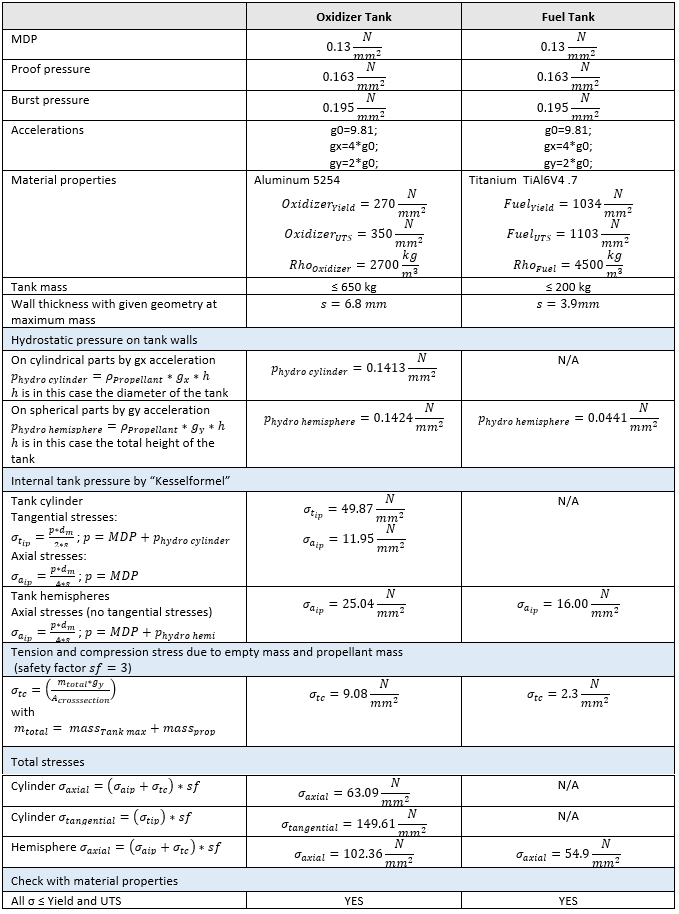
\includegraphics[width = 0.95\linewidth]{tankstress}
    \caption{Preliminary tank stresses calculation}\label{tab:tankstress}
\end{table}{}
\subsection{Liner tanks}
\subsubsection{Helium liner tank}

Only the fuel tank is pressurized by Helium and only needs a tank pressure of 1.3bar. The H2O2 tank is self-pressurizing due to the decomposing characteristics of H2O2. The specification of the helium liner tank is shown in \autoref{tab:helium}
\begin{table}[H]
    \centering
    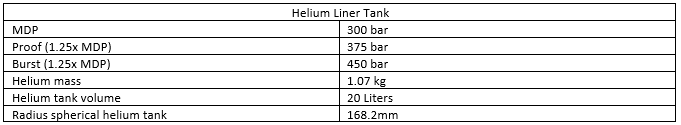
\includegraphics[width = \linewidth]{heliumliner}
    \caption{Helium liner tank specification}\label{tab:helium}
\end{table}{}
\subsubsection{$H_2$ liner tank}
The H2 is needed for the fuel cell. The specification of the h2 liner tank is shown in \autoref{tab:h2liner}.
\begin{table}[H]
    \centering
    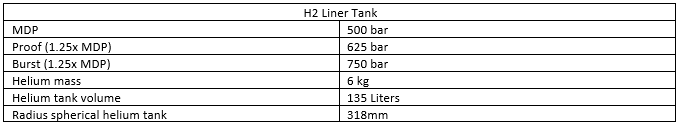
\includegraphics[width = \linewidth]{h2liner}
    \caption{Helium liner tank specification}\label{tab:h2liner}
\end{table}{}

\section{Catalyzer}
Besides the advantages of $H_2O_2$ there is one major drawback that we have to take into account. This drawback is that $H_2O_2$ needs to be decomposed in $H_2$ and $H_2O$ in order to react with RP-1. 

\begin{figure}[H]
	\centering
	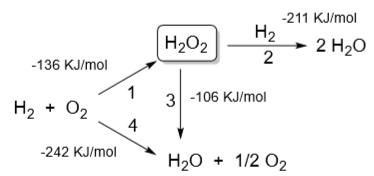
\includegraphics{H2O2}
	\caption{$H_2O_2$ chemical decomposition process}
\end{figure}

This decomposition is natural but at a low rate whereas we need a very high decomposition rate in order to feed the combustion chamber and sustain a proper flame. This decomposition is an exothermic decomposition. That's why we need a catalyser. \\

This catalyser needs to be placed between the turbo pump and the injectors. It allows to decompose the $H_2O_2$ at the last time. \\

The way a catalyser works is pretty simple; the $H_2O_2$ goes through a catalyst bed of silver pellets, reacts and generates heat. 
Why silver ? We chose silver because is the mostly used catalyser for $H_2O_2$. However, a lot of other different material exists, like Platinum, Manganese or even Gold but these materials are rarely used due to their cost and also the fact that they need to be made in complex alloy in order to optimize the reaction. 

\begin{figure}[H]
	\centering
	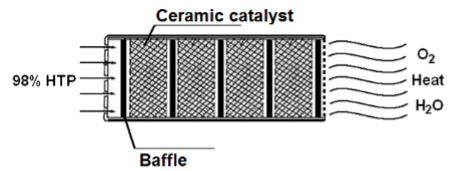
\includegraphics{catalyst}
	\caption{Example of catalyst bed}
\end{figure}

The figure above shows basically how a catalyser works. To have an idea of the shape of ours we just have to swap the ceramic catalyst by silver catalyst. So, it will be a steel cylinder filled with small spherical silver pellet separated by some baffles (silver grid mesh). \\

An important characteristic of the catalyser is the pressure drop it creates. This pressure drop influences the whole feeding system, the turbo pump sizing and even the injector design. that's why we need to characterize the pressure drop created by the catalyser. In order to do so, we are going to use the Ergun equation for packed bed reactor:

$$
\frac{\Delta p}{L} = 151.2 \frac{\mu}{d^2}\frac{(1-\epsilon)^2}{\epsilon^2}u + 1.8 \frac{\rho}{d}\frac{1- \epsilon}{\epsilon^3}u^2
$$

With $\mu$ the dynamic viscosity, $\epsilon$ the porosity, $d$ the pellet diameter, $\rho$ the density, $L$ the length of the bed and $u$ the velocity. \\

In this equation we need some important component such as $\epsilon$. The porosity is complicated to compute and need to be model. According to a recent research we determined a porosity of $0.3802$ with a pellet diameter of 5mm.

\begin{figure}[H]
	\centering
	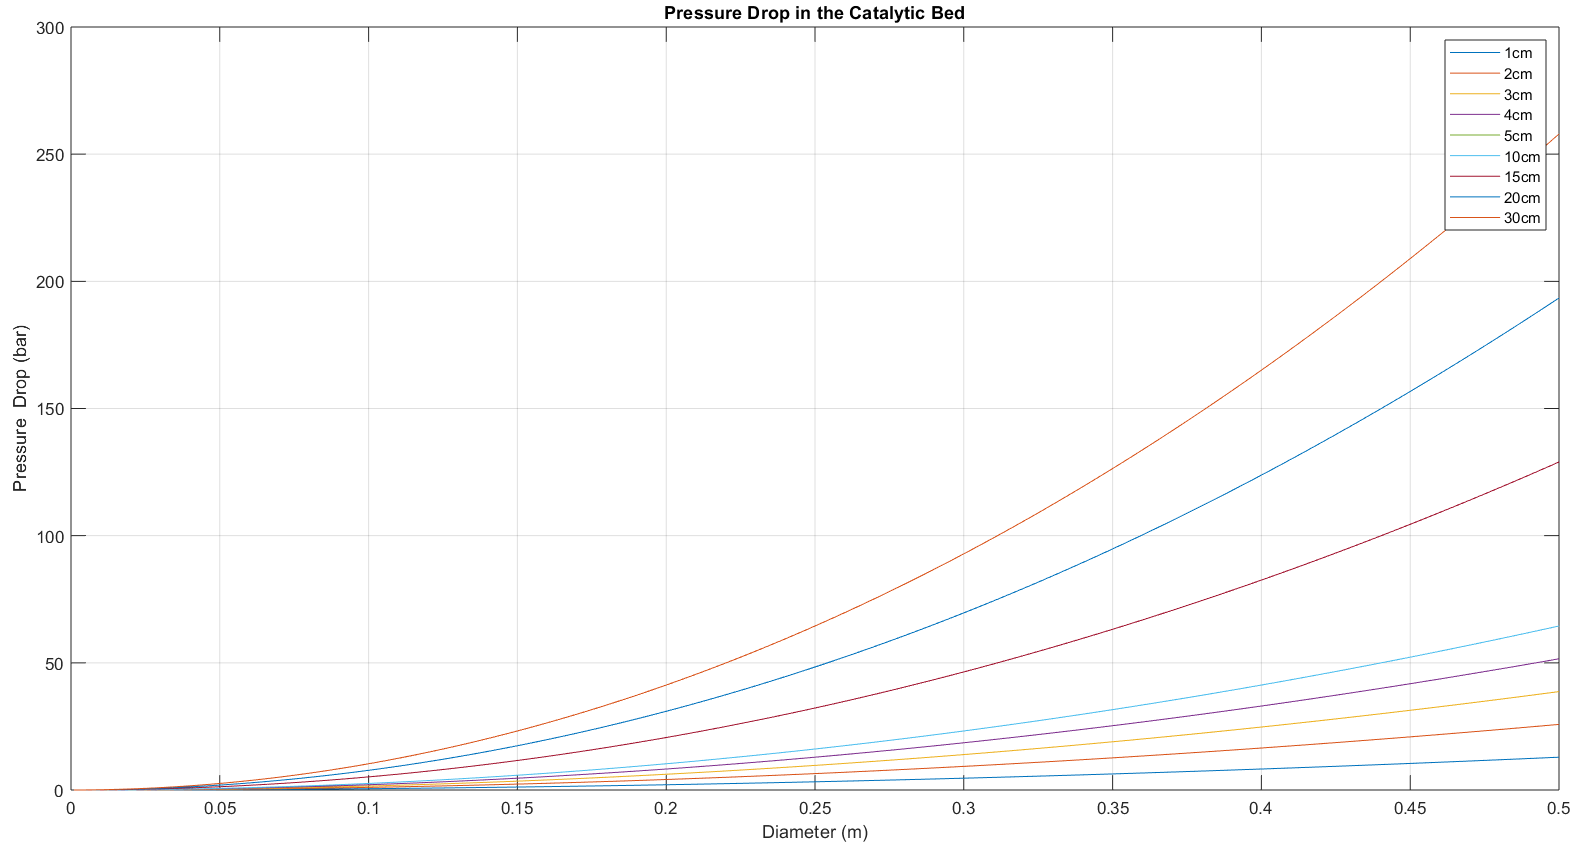
\includegraphics[width=\linewidth]{pressuredrop}
	\caption{Pressure drop depending on the size of the catalyst bed}
\end{figure}

We see on the graph that the pressure drop rise quickly with the size of the bed. So we need to limit the size of our catalyser in order to not oversize the turbo pump. To do so, we chose to limit our pressure drop to around 30 bars. Finally we obtain a cylinder of 20 cm of diameter and 20 cm of length. \\

This geometry allows the catalyser to provide a sufficient decomposition rate, a "contained" pressure drop and size. It also generates a great heat as high as $1000K$ at the exit of the catalyst bed. 

\section{Injectors}

To design our injectors we made some research and went through the literature about injector for hypergolic injector. We found interesting results in this paper\footnote{The design and main performance of a hydrogen peroxide/kerosene coaxial-swirl injector in a lab-scale rocket engine (2017)}. Their goal was to design a small attitude control system hydrogen peroxide/RP-1 thruster, to do so they compared two main different kind of injectors; the coaxial shear injector and the coaxial-swirl injector. \\

After simulation the results were that coaxial shear causes the combustion chamber to be divided into three different zones, these zones are: rapid high-temperature pyrolysis, oxidization and equilibrium flow. This kind of separation can cause serious bad behaviors during the combustion process and creates issues like flame-out, explosion or very poor efficiency. \\
In order to avoid these kind of behaviors the use of swirl-coaxial injectors is the best choice to make. \\

The concept of the swirl injector is pretty simple. Indeed, it's based on a coaxial injection but instead of injecting the two propellant in the axis of the injector, here the two propellant are injected radially in what is called the vortex chamber. 
The radial injection combine with the chamber allows to create a vortex of $H_2O_2$ and RP-1 which result in a generation of a plume of propellant at the exit of the injector. In addition, due to the geometry of such an injector, the reduction of diameter at the exit, the atomization is very easy.

\begin{figure}[H]
    \centering
    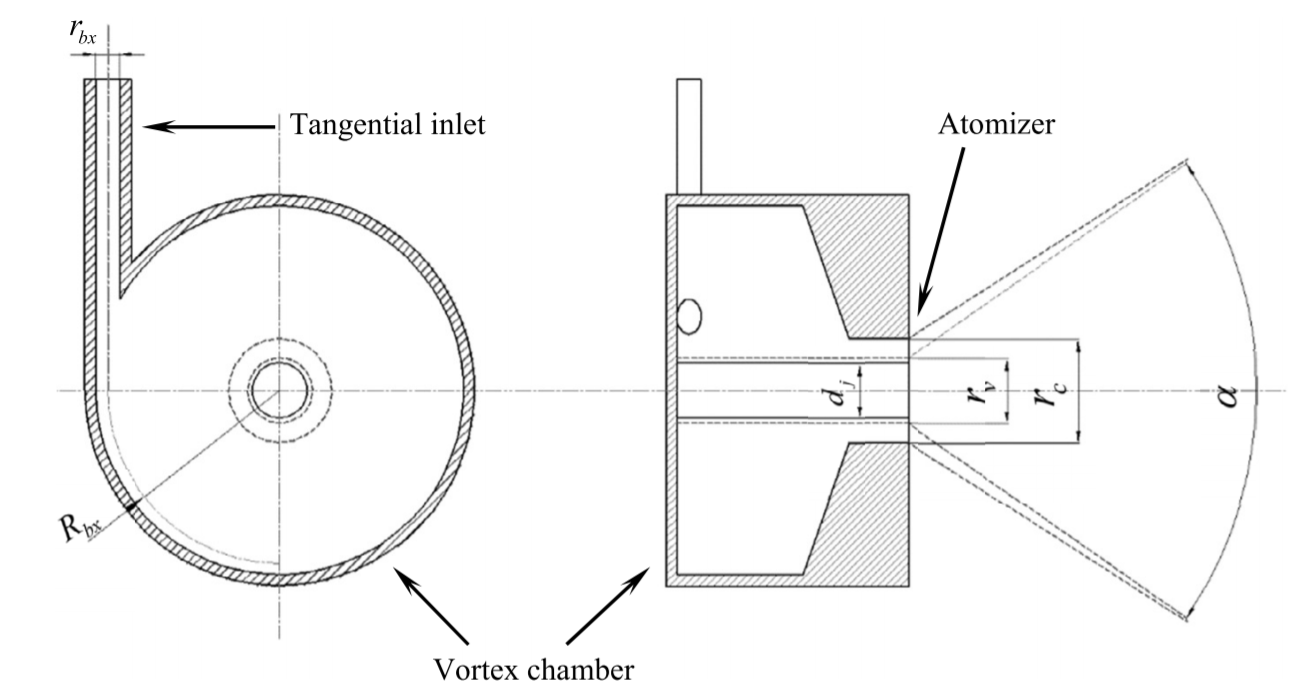
\includegraphics[width=\linewidth]{swirl}
    \caption{Cross section of a swirl injector}
\end{figure}

The schematic before shows how a swirl injector works. We see that there is only few parameters to take into account to design this kind of injector. These different parameters will be explain later on. \\

Our injection will be a liquid-gas injection but this characteristic is not really a problem for a swirl injector as the two propellant will behave the same way as a liquid or a gas.\\

in addition of these advantages the swirl injector offers an other non-negligible advantages that it allow us to improve our efficiency. Indeed, the study show that a swirl injector increases the combustion stability and efficiency up to 10$\%$ which result in a better fuel consumption during the operating time of the spacecraft. 


\section{Feeding system}
After having designed most of our propulsion system. We need to carefully link them by designing our feeding system. The biggest challenge is to create a system that will both fit in our spacecraft and deliver the right amount of propellant from the tanks to the engine through our different, required other subsystems.\\

The general pressure loss in a system is given by :

$$
\Delta P = K\frac \rho 2 w^2
$$

With $K$ depending on the type of change in system geometry as follow : 
\begin{figure}[H]
	\centering
	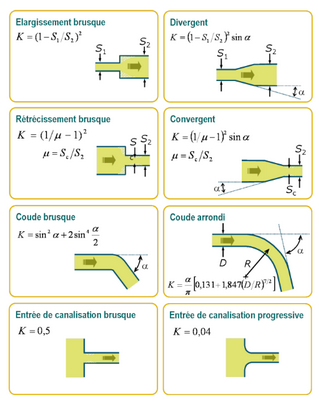
\includegraphics[height=12cm]{pertecharge}
	\caption{$K$ values for geometry changes}
\end{figure}
In our case, we will use the progressive line entering loss $K = 0.04$ and the bends $ K(\alpha) = \sin^2(\alpha) + 2\sin^4\bigg(\frac\alpha 2\bigg)$. Another $K$ will also be used for the entrance of the injector, which will be specified later on.\\

For manufacturing costs and simplicity purposes, we choose to only use $45^\circ$ bends which will result in $K_{bends}=0.5429$.\\

With that and the length measurements in mind, we designed the following feeding system layout for which we will then calculate the pressure variations along it :
\begin{figure}[H]
	\centering
	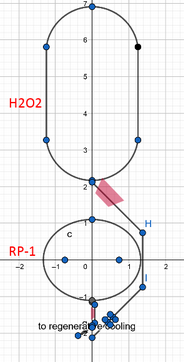
\includegraphics[height=10cm]{feeding}
	\caption{Feeding system layout (To scale)}
\end{figure}
\begin{figure}[H]
	\centering
	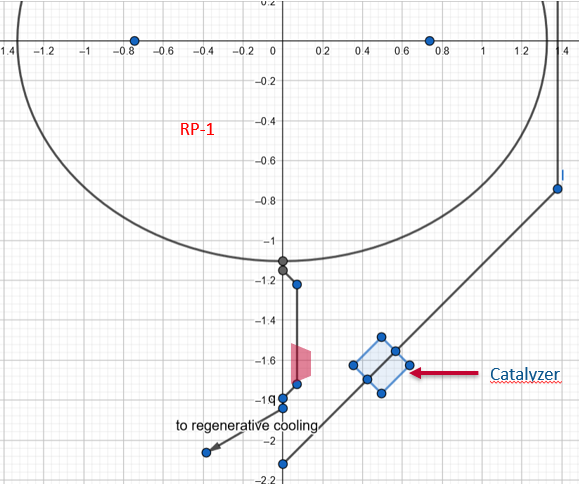
\includegraphics[height=8cm]{feedingzoom}
	\caption{Feeding system layout - Zoomed (To scale)}
\end{figure}
\subsection{Line diameters}
In order to choose our line diameters, we can first use our volume flow and then get the line area from it and then at the end, the line diameter.\\
\underline{Fuel} 
\begin{align}
\dot{V_f}&= \frac{\dot{m_f}}{\rho_f} = 0.0015298m^3/s\\
A_{line_f} &= \frac{\dot V_f}{w_f}=5.21\times 10^{-5} mm^2\\
d_{line_f} &= 2\sqrt{\frac{A_{line_f}}{\pi}} = 8.1447mm
\end{align}
As we are trying to insure a high injection velocity and to insure a certain margin in pressure and velocity, we will choose a line diameter of $7$ mm for the fuel feeding system.
\underline{Oxidizer}
\begin{align}
\dot{V_o}&= \frac{\dot{m_o}}{\rho_o} = 0.006042m^3/s\\
A_{line_o} &= \frac{\dot V_o}{w_o}=0.000275 mm^2\\
d_{line_o} &= 2\sqrt{\frac{A_{line_o}}{\pi}} = 18mm
\end{align}
In this case, we will choose a line diameter of $15$ mm for the oxidizer.

\subsection{Fuel feeding system}
The following items in our fuel feeding system will cause pressure drops :
\begin{itemize}
	\item Tank exit : $K=0.04$
	\item 4 $\times$ $45^\circ$ bends : $K = 0.5429$ for each
	\item Straight line losses : $\Delta P = \frac \rho 2 w^2 f \frac{L}{D}$
	\item Friction coefficient : $f = 0.02$
	\item Regenerative cooling : $\Delta P = 0.25$ bar
	\item Fuel injection : $\Delta P = 9.3843$ bars
\end{itemize}

With our current layout, we have $5$ straight lines which will cause pressure losses on the fuel side. Three of them are before the turbopump which is placed at the end of the third straight section, right before the third bend. We consider a velocity of $8$ m/s before the turbopumps and of $v_{inj}=29.363$ m/s after. The line loss for each section is given by : 
$$
\Delta P = \frac {810} 2 w^2 \times 0.02 \times \frac{L_{section}}{0.007}
$$
\begin{enumerate}
	\item First section ($L_{section}=0.05m$) : $\Delta P = 0.037029$ bar
	\item Second section ($L_{section}=0.1m$) : $\Delta P = 0.074057$ bar
	\item Third section ($L_{section}=0.5m$) : $\Delta P = 0.37029$ bar
	\item Fourth section ($L_{section}=0.1m$) : $\Delta P = 0.997699$ bar
	\item Fifth section ($L_{section}=0.05m$) : $\Delta P = 0.49884$ bar
\end{enumerate}
There are also two different values for the bend losses depending on the position of the bend (before or after the turbopump), we have $2$ of each :
\begin{itemize}
	\item $\Delta P_{before} = 0.14072 $ bar
	\item $\Delta P_{after} = 1.8957$ bar
\end{itemize}
The tank exit loss is :
$$
\Delta P_{exit} = K_{exit} \times \frac{\rho_F}2 \times 8 ^ 2 = 0.010368\text{ bar}
$$
\subsection{Oxidizer feeding system}
The following items in our oxidizer feeding system will cause pressure drops :
\begin{itemize}
	\item Tank exit : $K=0.04$
	\item 4 $\times$ $45^\circ$ bends : $K = 0.5429$ for each
	\item Straight line losses : $\Delta P = \frac \rho 2 w^2 f \frac{L}{D}$
	\item Friction coefficient : $f = 0.02$
	\item Catalyzer : $\Delta P = $ bars
	\item Oxidizer injection : $\Delta P = 4.9599$ bars
\end{itemize}

On this part of the feeding system, we also have $5$ sections and $4$ bends of $45^\circ$ each. We also consider a velocity of $8$ m/s before the turbopump and $21.971$ m/s after. However, due to the larger distances (due to our tank layout), the turbopump's position in the feeding system is different and is now positioned after the first bend, right at the beginning of the second straight line. This results in $3$ bends being at high velocity and $1$ at relatively slower velocity.\\

Here, each straight line loss section is given by : 
$$
\Delta P = \frac {1450} 2 w^2 \times 0.02 \times \frac{L_{section}}{0.015}
$$
With : 

\begin{enumerate}
	\item First section ($L_{section}=0.05m$) : $\Delta P = 0.030933$ bar
	\item Second section ($L_{section}=1.95m$) : $\Delta P = 9.0992$ bars
	\item Third section ($L_{section}=1.4836m$) : $\Delta P = 6.9228$ bars
	\item Fourth section ($L_{section}=1.15m$) : $\Delta P = 5.3662$ bars
	\item Fifth section ($L_{section}=0.6m$) : $\Delta P = 2.7997$ bars
\end{enumerate}

For the bends, we have :

\begin{itemize}
	\item $\Delta P_{before} = 0.2519 $ bar ($1$ of them)
	\item $\Delta P_{after} = 1.0614$ bar ($3$ of them)
\end{itemize}

The tank exit loss is :
$$
\Delta P_{exit} = K_{exit} \times \frac{\rho_o}2 \times 8 ^ 2 = 0.01856\text{ bar}
$$
\section{Turbo pumps}
As most of our subsystems have a defined pressure drop due to their specific design, we have made the choice to use this feeding system design with all losses included to then design our turbopumps to have a pressure rise in accordance with our pressure requirements. We chose to go with electrically driven turbo pumps as we have a good amount of electrical power since we use fuel cells in our spacecraft.\\

Our respective turbopump required created pressures are : 
\begin{itemize}
	\item Fuel side : $\Delta P_{T_f} = P_{Chamber} + \Delta P_{feeding_f} + \Delta P_{inj_f} + \Delta P_{Regenerative\ cooling} - P_{Tank_f}$
	\item Oxidizer side : 	$\Delta P_{T_o} = P_{Chamber} + \Delta P_{feeding_o} + \Delta P_{inj_o} + \Delta P_{Catalyzer} - P_{Tank_o}$
\end{itemize}
Thus,
\begin{align}
\Delta P_{T_f} &= 54.395\ \text{bars}\\
\Delta P_{T_o} &= 102.28\ \text{bars}
\end{align}
Considering an efficiency of $0.9\times 0.75$, with $0.9$ for the electrical part and $0.75$ for the mechanical part, we get the following powers :
\begin{align}
	Power_{fuelpump} &=\dot{m_f}\frac{P_{T_f}}{\rho_F \eta} = 13\ 461\ W\\
	Power_{Oxpump} &= \dot{m_o}\frac{P_{T_o}}{\rho_o \eta} = 96\ 030\ W
\end{align}
Considering a maximum continuous burn time of $900$ seconds, we get the following energy with a 40\% margin as we are still unsure about the performance of such turbopump :\\
\begin{equation}
	E_{kWh} = \frac{(Power_{fuelpump} + Power_{Oxpump})\times 900}{3.6\times 10^6} = 38.322\ kWh
\end{equation}

We also know the following vapor pressures :
\begin{itemize}
	\item $H_2O_2$ : $666.612$ Pa at $30^\circ$ C
	\item $RP-1$ : $700$ Pa between $20^\circ$C and $25^\circ$ C
\end{itemize}
With the information we have, we can calculate the pump head rise and the NPSH.
\begin{align}
	H_{p_{Fuel}} &= \frac{\Delta p_{p_{Fuel}}}{g_0 \rho_{Fuel}} = 747.474\ m\\
	H_{p_{Ox}} &= \frac{\Delta p_{p_{Ox}}}{g_0 \rho_{Ox}} = 754.192\ m\\
	NPSH_{Fuel} &= \frac{p_{i_{Fuel}} - p_{v_{Fuel}}}{g_0 \rho_{Fuel}} = 6.569\ m\\
	NPSH_{Ox} &= \frac{p_{i_{Ox}} - p_{v_{Ox}}}{g_0 \rho_{Ox}} = 7.0465\ m
\end{align}
We can then get the number of stages :
\begin{equation}
	n= 1 +floor(\frac{\Delta p_p}{\Delta p_{ps}})
\end{equation}
Thus, using $\Delta p_{ps} = 47\times 10^6\ Pa$,
\begin{align}
	n_{Fuel} &= 126\ 373
	n_{Ox} &= 228\ 256
\end{align}
We can also get the rotation speeds :
\begin{align}
	N_{Fuel} &= 1.636\ rad/s = 15.623\ RPM\\
	N_{Ox} &= 0.532\ rad/s = 5.079\ RPM
\end{align}
Then
\begin{align}
	u_{t_{Fuel}} &= \sqrt{\frac{gH_{p_{Fuel}}}{n\psi}}=0.325\ m/s\\
	u_{t_{Ox}} &= \sqrt{\frac{gH_{p_{Ox}}}{n\psi}} =0.243\ m/s\\
	D_{2t_{Fuel}} &=\frac{u_{t_{Fuel}}}{N_{r_{Fuel}}}= 0.199\ m\\
	D_{2t_{Ox}} &= \frac{u_{t_{Ox}}}{N_{r_{Ox}}} 0.457\ m\\
	D_{1t_{Fuel}} &= \sqrt[3]{\frac{\frac{4}{\pi}Q_{Fuel}}{\phi N_{r_{Fuel}}(1-L^2)}} = 2.197\ m\\
	D_{1t_{Fuel}} &=\sqrt[3]{\frac{\frac{4}{\pi}Q_{Ox}}{\phi N_{r_{Ox}}(1-L^2)}} = 6.131\ m
\end{align}
\section{Pressure evolution summary}
\subsection{Fuel side}
\begin{table}[H]
	\centering
\begin{tabular}[H]{|c|c|c|}
	\hline
	\cellcolor{gray!50}Contributor& \cellcolor{gray!50}Pressure Drop (bars) & \cellcolor{gray!50}Pressure at the end of this part (bars)\\
	\hline
	Tank & NA & $1.3$ \\
	\hline
	Tank exit & $0.010368$ & $1.29$\\
	\hline
	First section & $0.037$ &$1.253$\\
	\hline
	First bend &$0.14$ &$1.113$\\
	\hline
	Second section &$0.074$ &$1.039$\\
	\hline
	Second bend &$0.14$ &$0.899$\\
	\hline
	Third section &$0.37$ &$0.529$\\
	\hline
	Turbo pump & $54.395 $ (Rise) &$59.924$\\
	\hline
	Valve & $5$ &$54.924$\\
	\hline
	Third bend &$1.8957$ &$53.0283$\\
	\hline
	Fourth section &$0.997$ &$52.0313$\\
	\hline
	Fourth bend &$1.8957$ &$50.1356$\\
	\hline
	Fifth section &$0.499$ &$49.6366$\\
	\hline
	Cooling &$0.25$ &$49.3866$\\
	\hline
	Injection &$9.38$ &$40.0066$\\
	\hline
	Combustion chamber & NA &$40.0066$\\
	\hline
\end{tabular}
\caption{Pressure evolution on fuel side}
\end{table}
\begin{figure}[H]
	\centering
	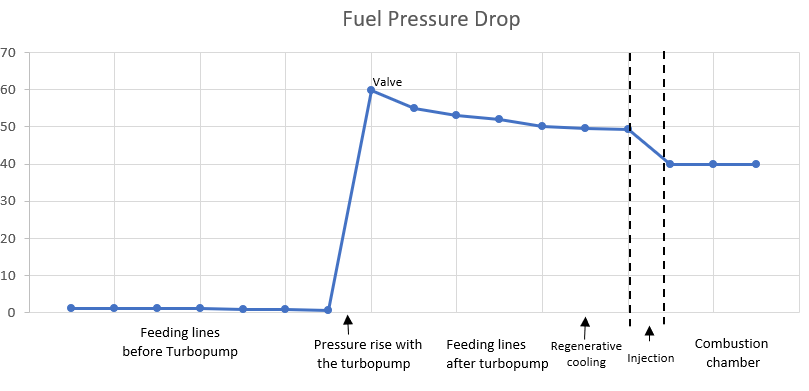
\includegraphics[width=\linewidth]{fuelchart}
	\caption{Pressure evolution on fuel side (bars)}
\end{figure}
\subsection{Oxidizer side}
\begin{table}[H]
	\centering
\begin{tabular}[H]{|c|c|c|}
	\hline
	\cellcolor{gray!50}Contributor& \cellcolor{gray!50}Pressure Drop (bars) & \cellcolor{gray!50}Pressure at the end of this part (bars)\\
	\hline
	Tank & NA & $1.3$ \\
	\hline
	Tank exit & $0.010368$ & $1.29$\\
	\hline
	First section & $0.031$ &$1.259$\\
	\hline
	First bend &$0.25$ &$1.009$\\
	\hline
	Turbo pump & $102.28 $ (Rise) &$108.289$\\
	\hline
	Turbo pump & $5$ &$103.289$\\
	\hline
	Second section &$9.09$ &$94.199$\\
	\hline
	Second bend &$1.06$ &$93.139$\\
	\hline
	Third section &$6.9228$ &$86.2162$\\
	\hline
	Third bend &$1.06$ &$85.1562$\\
	\hline
	Fourth section &$5.366$ &$79.7902$\\
	\hline
	Fourth bend &$1.06$ &$78.7302$\\
	\hline
	Fifth section &$2.7997$ &$75.9305$\\
	\hline
	Catalyzer &$30.95$ &$44.9805$\\
	\hline
	Injection &$4.96$ &$40.0205$\\
	\hline
	Combustion chamber & NA &$40.0205$\\
	\hline
\end{tabular}
\caption{Pressure evolution on fuel side}
\end{table}
\begin{figure}[H]
	\centering
	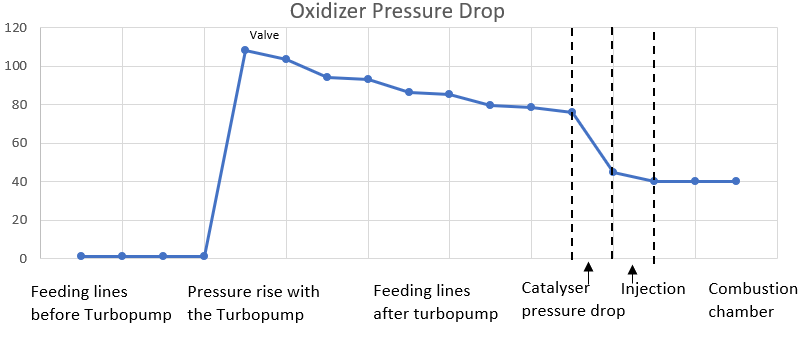
\includegraphics[width=\linewidth]{oxchart}
	\caption{Pressure evolution on oxidizer side (bars)}
\end{figure}
\section{Engine}
\section{Nozzle}
